\chapter{Identification du Sens du Résultat par Classification}
\label{chap:sensresultat}

\section{Objectif et Motivation}
\label{sec:sensresultat:motivation}
Comme le précédent, ce chapitre est relatif à l'extraction de données sur les demandes, mais  il est question ici d'extraire uniquement le sens du résultat d'une demande connaissant sa catégorie. Cette étude est intéressante parce que le problème devient plus simple. En se passant de la localisation précise des quanta ou plus globalement des passages d'expression des demandes et résultats, l'extraction du sens du résultat peut être formulée comme une tâche de classification de documents. Nous modélisons la tâche comme une classification binaire où un algorithme est entraîné à déterminer si la demande a été rejetée (sens = rejette) ou acceptée (sens = accepte). Nous avons proposé cette modélisation sur une restriction du problème définie par les postulats \ref{postulat:sens:unedemande} et \ref{postulat:sens:sensbinaire}.

\begin{postulat}\label{postulat:sens:unedemande}
Pour toute catégorie de demande $C$, la majorité des documents ne contiennent qu'une demande de catégorie $C$.
%Pour toute catégorie de demande $C$, on ne considère que les décisions dans lesquelles n'apparaît qu'une seule demande de catégorie $C$. 
\end{postulat} 
Ce postulat est légitime car les statistiques sur les données labellisées de la Figure \ref{fig:quanta:hist-repartition-docs} montre bien que pour la majorité des catégories, peu de décisions contiennent plus d'une demande. On remarque néanmoins l'exception de la catégorie STYX (dommage-intérêt sur l'article 700 CPC), où dans la majorité des documents, on a plutôt 2 demandes. Cette exception peut se justifier par le fait que chaque partie fait généralement ce type de demande car elle porte sur le remboursement de frais de justice. Ce postulat présente cependant un inconvénient dû au fait que la majorité des demandes se trouvent dans des décisions à plus d'une demande. Il est donc possible de manquer un grand nombre de demandes. %On pourrait peut-être porter la classification à un modèle multi-label qui déterminera plusieurs sens à partir d'un seul document. Par exemple <SENS1, SENS2, SENS3> avec des valeurs prédéfinies sur les SENS 2 et 3 par exemple NO-DMD pour indiquer que la décision ne comprend pas de seconde ou de troisième demande.

\begin{postulat}\label{postulat:sens:sensbinaire}
Le sens du résultat est généralement binaire: accepte ou rejette.
\end{postulat} 
Ce postulat est justifié car le sens d'un résultat est pratiquement toujours une de ces deux valeurs (Figure \ref{stat-sensrst}). Les autres sens étant très rares, nous ne les considérons pas.

\begin{figure}
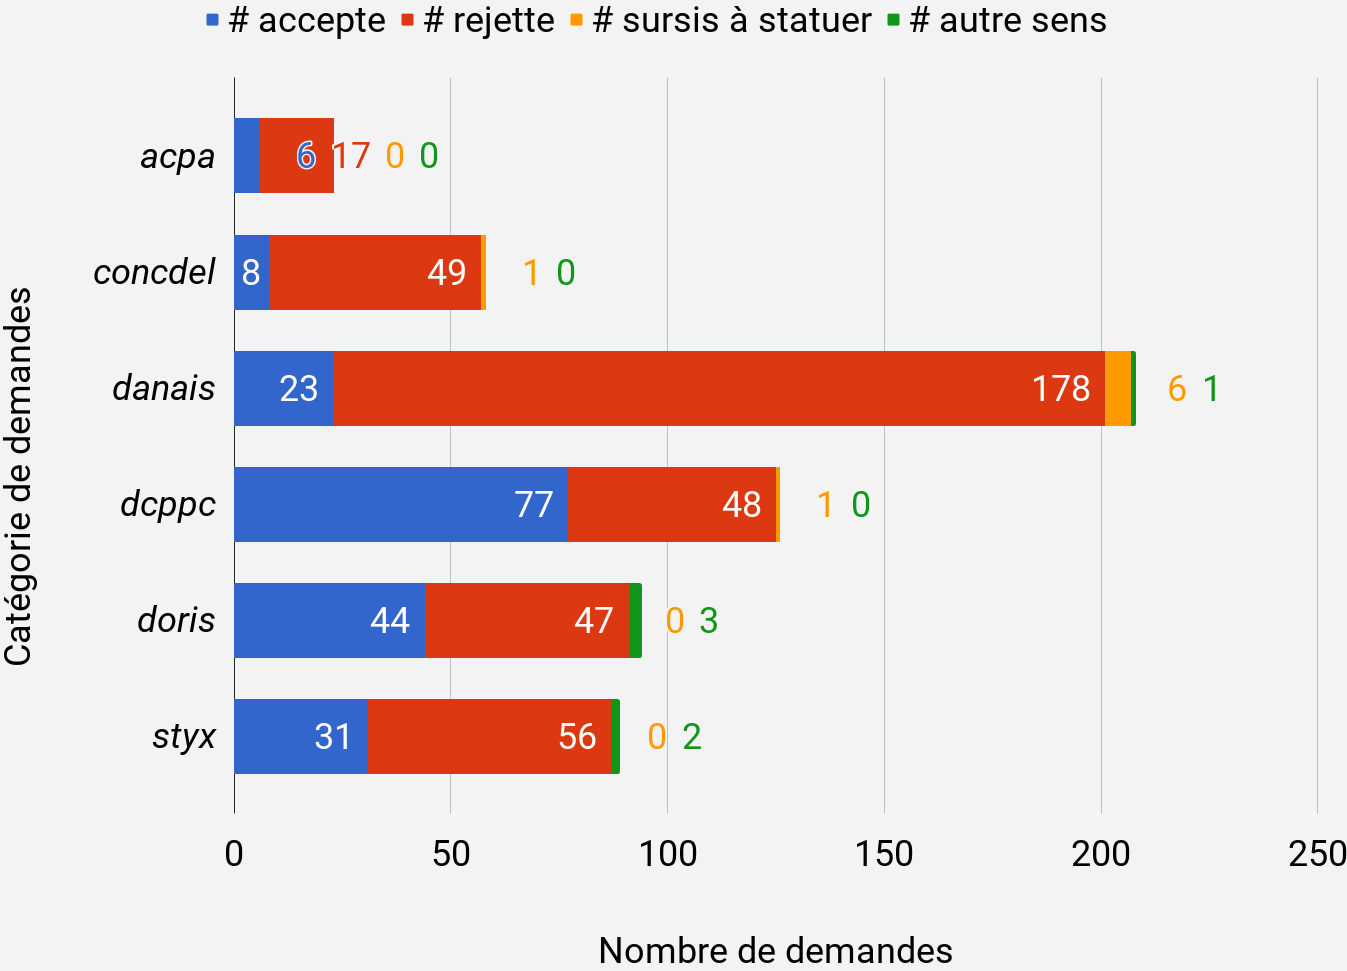
\includegraphics[width=\textwidth]{chartDistrSens.png}
\caption{Répartition des sens de résultat dans les données annotées.}\label{stat-sensrst}
\end{figure}
\section{Formulation du Problème}
\label{sec:sensresultat:probleme}

Cette étude porte sur l'analyse de l'impact de différents aspects techniques généralement appliqués dans le cadre de la classification de texte:
La représentation de texte (généralement vectorielle) faisant intervenir les notions de BagOfWord, TFIDF, poids global, poids local, matrice document-terme
La transformation de dimension a pour but de projeter le vecteur représentant un document dans un nouvel espace où généralement la distinction des classes est plus facile. Ceci est généralement effectuée en déterminant des composantes discriminantes à partir de la base d'entraînement: sélection de caractéristique, réduction matricielle, représentation vectorielle “sémantique” des documents (LatentDA, LSA, word embedding, ...)

 Cette analyse permettra de savoir s'il existe une certaine configuration permettant de déterminer le sens du résultat à une demande sans nécessairement l'avoir identifiée précisément dans le document. 


\section{Classification de Documents}
\label{sec:sensresultat:biblio_classif}

La classification de texte permet d'organiser des documents $x^{(k)}$ dans des groupes prédéfinis. Elle reçoit depuis longtemps beaucoup d'attentions. Deux choix techniques influencent principalement les performances: la représentation des textes et l'algorithme de classification. 

\subsection{Algorithmes traditionnels}
Bien que la classification de documents voit de plus en plus se développer des algorithmes propres aux textes, un grand nombre de méthodes ont été développées précédemment autour. Ces méthodes sont généralement basée sur une représentation vectorielle des textes et délimitent une frontière entre les classes dans un espace multidimensionnel. 
%NB et SVM : https://www.dropbox.com/home/Documents/to-read/term-weight?preview=Best+Terms+An+Efficient+Feature+Selection+Algorithm+for+Text+Categorization.pdf

\subsection{Etat de l'art}
Actuellement, les algorithmes NBSVM et FastText sont les plus populaires pour la classification de documents et ont les performances pour l'analyse de sentiment sont très bonnes. 

Le NBSVM \citep{wang2012nbsvm} est un classifieur binaire (classes $\lbrace -1; 1 \rbrace$) dont le principe consiste à transformer les poids $f^{(k)}$ caractéristiques $V$ des textes $x^{(k)}$, réduites à leur simple présence $\widehat{f}^{(k)}$ en réalisant leur produit élément à élément ($\overset{\sim}{f}^{(k)} = {r} \circ \widehat{f}^{(k)}$) avec le vecteur de poids $r$ du classifieurs bayésien multinomial (calculé avec le vecteur présence de caractéristique):
$r = \log \left( \frac{p/\vert\vert p \vert\vert_1}{q / \vert\vert q \vert\vert_1}\right)
\text{ avec } p=\alpha + \sum\limits_{k:y^{(k)}=1}{f}^{(k)}$, $q=\alpha + \sum\limits_{k:y^{(k)}=-1}{f}^{(k)}$. L'ensemble des caractéristiques $V$ est constitué de n-grammes de mots. Le nouveau vecteur issu de ce produit représente le texte ($x^{(k)} = \overset{\sim}{f}^{(k)}$) en entrée d'un SVM classique. La classe de $x^{(k)}$ est prédite par : $y^{(k)} = sign(\mathbf{w}^Tx^{(k)} + b)$, $\mathbf{w}$ et $b$ étant appris lors de l'entrainement du SVM. Une interpolation  entre le bayésien multinomial et le SVM est nécessaire pour assurer la robustesse du NBSVM et des performances excellentes pour toute tâche de classification de documents; les poids $\mathbf{w}$ sont réajustés par le model $\mathbf{w'} = (1 - \beta) \overline{w} + \beta \mathbf{w}$, où $\overline{w} = \vert\vert \mathbf{w}\vert\vert_1 / \vert V \vert$ et $\beta \in \left[0; 1] \right.$. 
  
 FastText \citep{grave2017fasttextcls}, quant à lui, est un modèle de réseau de neurones dont l'architecture est semblable à celle de la variante CBOW de la méthode de plongement sémantique Word2Vec dans laquelle le mot du milieu a été remplacé par le label de la classe du texte et au dessus de laquelle la fonction softmax $f(z) = \left[ \frac{e^{z_j}}{\sum\limits_{k=1}^K e^{z_k}} \right]_{\forall j \in \lbrace 1, ..., K \rbrace} $ est rajoutée pour réaliser la classification à partir de la représentation distribuée du texte. La phase d''entraînement consiste à minimiser la fonction objectif $-\frac{1}{N}y_n \cdot \sum\limits_{n=1}^N y_n \cdot \log{f(B\cdot A\cdot x_n)}$ qui estime la distribution de probabilité des classes.

Le fonctionnement de ces deux méthodes intègrent leur propre représentation, contrairement aux algorithmes traitant des vecteurs comme le SVM. Il existe un très grand nombre de schémas de représentations vectorielles des documents.

NBSVM et Fastext ont démontré une bonne robustesse et et des performances excellentes dans le cas de divers tâches de classification: courtes expressions, longs documents, thème, classification subjective (genre), classification de sentiment (positif, neutre, négatif), ... Mais nous voulons déjà savoir comment les algorithmes populaires se comportent sur notre tâche d'identification de la polarité du résultat d'une demande pour une catégorie bien définie. La particularité ici est que la tâche porte sur une demande en particulier parmi les nombreuses que compte le document, des données en faible nombre annotés (23 à 189 documents), une annotation en général déséquilibrée entre les classes (risque d'ignorer une classe très faiblement représenté dans le jeu d'entrainement, par exemple 21 "accepte" contre 166 "rejette").

\subsection{Classification des décisions de justice}

\section{La Regression PLS et ses extensions}
\label{sec:sensresultat:pls}
\textcolor{red}{Justification: Pourquoi le PLS?:}
%https://link.springer.com/content/pdf/10.1007\%2FBF02174528.pdf, 
%https://www.stat4decision.com/fr/regression-pls/
La regression PLS est une méthode de regression avec laquelle l'on tente d'expliquer une ou plusieurs variables Y (dite dépendantes) par des variables $X=x_1,x_2,...,x_p$ (dites explicatives). Elle consiste principalement à transformer les variables explicatives en un nombre réduit de composantes principales orthogonales $t_1, t_2, ..., t_h$. Les composantes $t_h$ sont construites étapes par étapes en applicant l'algorithme du PLS de façon récurrente sur les données mal prédites (résidus). Plus précisément, à chaque itération $h$, la composante $t_h$ est calculée par la formule $t_h = w_{h1} x_1 + \cdots + w_{hj} x_j + \cdots + w_{hp} x_p$. 

Malgré quelques faiblesses comme celles liées au choix du nombre de composantes, à la complexité des sorties et la linéarité du modèle, la regression PLS présente quelques atouts qui ont notamment de l'intérêt dans notre cas de figure. Par exemple, le PLS gère assez bien la forte dispropotion entre le nombre de variables explicatives et le nombre d'observations, lorsque ce dernier est faible comme on peut l'observer dans nos données (faible quantité de données d'apprentissage). Nous avons aussi la prise en compte de la multicolinéarité qui peut exister entre les variables explicatives, notamment quand celles-ci sont associées aux mots/termes souvent cooccurrents de nos documents.

Il est intéressant de noter la floraison d'extensions proposées pour répondre aux différentes limites du PLS. Notamment, nous pouvons citer la "\textit{sparse}" PLS introduite pour palier à la "\textit{sparsité}" et la colinéarité des variables explicatives [?], la PLS non-linéaire proposée pour les cas de données non-linéairement séparables [?], ou encore la PLS discriminante combinant la régression PLS et l'analyse discriminante [?]. Nos nous sommes intéressés à deux extensions particulières: la régression Gini-PLS \citep{mussard2018ginipls} dont l'intérêt est de réduire la sensibilité aux valeurs aberrantes des variables, et la regression Logit-PLS \citep{tenenhaus2005logitpls}  combinant la regression logistique et la PLS.
\subsection{Gini-PLS}
Cette méthode élimine la sensibilité du PLS aux valeurs extrêmes en remplaçant la covariance $cov(x_j, y)$ par la covariance de Gini $cog(y; x_j) := cov(y; R(x_j))$ pour l'estimation des résidus $u_{(h)j}$ et des poids $w_{hj}$ \citep{mussard2018ginipls}.


\subsection{Logit-PLS}
Dans cette approche, $\forall j > 1$, les $w_{hj} $ sont les coefficients de la régression logistique de $y$ sur les composantes $t_1, ..., t_{h-1}, u_{(h-1)j}$ \cite{tenenhaus2005logitpls}.

\subsection{Gini-Logit-PLS}
Cette approche combine la covariance Gini pour $u_{(h)j}$ et le coefficient Logit pour les $w_{hj}$.

\section{Expérimentations et résultats}
\label{sec:sensresultat:experimentations}
\subsection{Protocole d'évaluation}
Nous discutons ici les performances de divers algorithmes populaires et l'impact de la quantité et du déséquilibre des données, de la restriction à des passages en particulier, aisin que leur capacité à faire abstraction des autres demandes du document. Deux métriques d'évaluation sont utilisées: la précision et la F1-mesure. Du fait du déséquilibre entre les classes, la moyenne des performances sur les deux classe sera micro (agrégation de la contribution individuelle de chaque classe: $F1_{moyenne} = (F1({accepte}) + F1({rejette})) / 2$).

Les données utilisées sont les mêmes que celles du chapitre précédent. Nous avons seulement fait une restriction sur les documents n'ayant qu'une seule demande annotée pour la catégorie considérée. Le déséquilibre entre les classes est illustrée par la figure \ref{fig:sensresultat:stat-1dmd}. En effet, la demande est plus souvent rejetée qu'acceptée pour les catégorie ACPA, CONCDEL, DANAIS et STYX. Le contraire est observé pour DCPPC et DORIS.
\begin{figure}[htb]
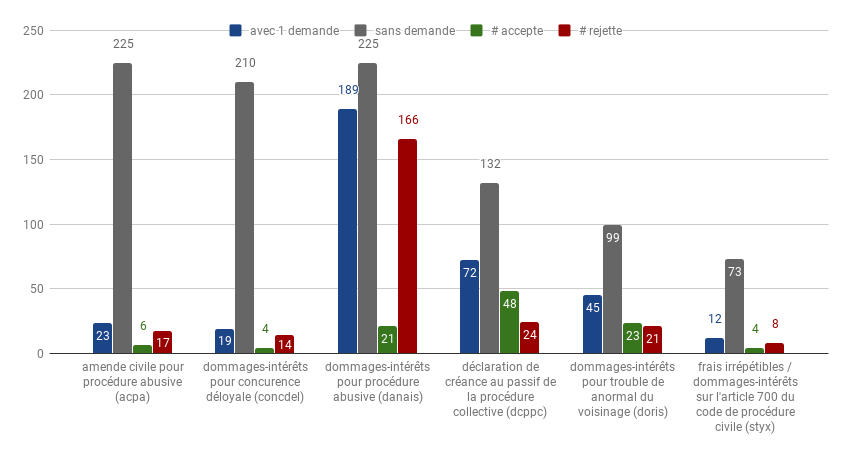
\includegraphics[width=\textwidth]{chartDataset1dmd.png}
\caption{Répartition des documents à une demande de la catégorie considérée.}\label{fig:sensresultat:stat-1dmd}
\end{figure}

\subsection{Performances observées}

\begin{table}
\scriptsize
\begin{tabular}{|l|l|l|l|l|l|l|l|l|}
\hline
\textbf{Cat. Dmd.} & \textbf{Algo.} & \textbf{Préc.}   & \textbf{Préc. équi.} & \textbf{err-0} & \textbf{err-1} & \textbf{f1-0}  & \textbf{f1-1}  & \textbf{f1-macro-avg} \\ \hline
\textbf{dcppc}       & nbsvm      & 0.875 & 0.812        & 0.375 & 0     & 0.752 & 0.916 & \textbf{0.834}        \\ \hline
danais      & fasttext   & \textbf{0.888} & 0.5          & 1     & 0     & 0     & 0.941 & 0.47         \\ \hline
danais      & nbsvm      & 0.888 & 0.5          & 0     & 1     & 0.941 & 0     & 0.47         \\ \hline
concdel     & fasttext   & 0.775 & 0.5          & 1     & 0     & 0     & 0.873 & 0.437        \\ \hline
concdel     & nbsvm      & 0.775 & 0.5          & 0     & 1     & 0.873 & 0     & 0.437        \\ \hline
acpa        & fasttext   & 0.745 & 0.5          & 1     & 0     & 0     & 0.853 & 0.426        \\ \hline
acpa        & nbsvm      & 0.745 & 0.5          & 0     & 1     & 0.853 & 0     & 0.426        \\ \hline
doris       & nbsvm      & 0.5   & 0.492        & 0.85  & 0.167 & 0.174 & 0.63  & 0.402        \\ \hline
dcppc       & fasttext   & 0.667 & 0.5          & 0     & 1     & 0.8   & 0     & 0.4          \\ \hline
styx        & fasttext   & 0.667 & 0.5          & 1     & 0     & 0     & 0.8   & 0.4          \\ \hline
styx        & nbsvm      & 0.667 & 0.5          & 0     & 1     & 0.8   & 0     & 0.4          \\ \hline
doris       & fasttext   & 0.523 & 0.5          & 0     & 1     & 0.686 & 0     & 0.343        \\ \hline
\end{tabular}
0 == accepte

1 == rejette

\caption{Performances des classifieurs pour l'identification du sens du résultat} \label{tab:sensresultat:perf-base}
\end{table}



\subsection{Discussions}
\subsubsection{Déséquilibre des classes}
\subsubsection{Quantités de données annotées}
\subsubsection{Restriction à une région particulière du document}
\subsubsection{Représentation des documents}

\section{Conclusion}
\label{sec:sensresultat:conclusion}